\chapter{Modeling Methodology}
\label{chap:procedure}
In this chapter, the methodology for the creation of the two models will be described.
\section{Procedure for Modelling of Global Model}
\label{sec:globmod}
The global model was created in SIMA RIFLEX, and consists of the whole cable attached to a point that will behave like the vessel due to the transfer functions provided from Dr. Techn. Olav Olsen. The following section will describe how the central properties of the cable were modeled in the numeric model. 

\subsection{Cross Sectional Properties}
The cable in the global model consists of two different cross sections, with the properties presented in table \ref{table:crosssima}. 
\begin{table} [H]
\centering
\begin{tabular}{ |c|c|c|}
\hline
Property& Cable Cross Section & Buoy Cross Section \\
 \hline
 \hline
Dry mass+ Buoyancy [$\frac{kg}{m}$] & 15.75 & 15.75\\
External Area [m]& 0.006171 & 0.03\\
Axial Stiffness [N] & 2.0e+08 & 2.0e+08\\
Bending Stiffness [Nm$^2$] & 1481 & 1481\\
Torsional Stiffness [Nm$^2$] & 5403 & 5403\\
 \hline
\end{tabular}
\caption{Parameters used for the two different cross sections}
\label{table:crosssima}
\end{table}
\noindent The only difference between the two is the external area due to the buoyancy elements attached to the buoy section. The parameters in table \ref{table:crosssima} were calculated as follows:\newline
\newline 
\noindent The mass coefficient: 
\begin{equation}
\text{Mass coeff.}=L_{c} A_cn_c (\rho_c-\rho_w) + L_{s1} A_{s}n_{s1} (\rho_s-\rho_w)+L_{s2} A_{s2}n_{s2} (\rho_s-\rho_w)
\end{equation}

\noindent Where $L_c$ is the length of a helical copper conductor pr meter, $A_c$ is the area of a copper conductor, $n_c$ is the number of copper conductors, $\rho_c$ is the density of copper, $\rho_w$ is the density of water, $L_{si}$ is the length of steel armouring pr meter for layer i, $A_s$ is the area of one wire for the steel armouring assumed to be the same for layer 1 and 2, $n_{si}$ is the number of wires in armouring layer i and $\rho_s$ is the density of steel. The plastic sheaths and tape were assumed to have the same density as the water. \newline
\newline 
The Axial stiffness and torsional stiffness was calculated according to equation 4.14 and 4.22 in \cite{Savik2016} as:
\begin{equation}
    EA=nEA_t \cos\alpha(\cos^2\alpha-\nu_a \sin^2\alpha)
\end{equation}

\begin{equation}
    GI=nA_t E R^2 \sin^2 \alpha \cos^2 \alpha
\end{equation}
Where $n$ is the number of wires in the steel armouring, $E$ is Young's modulus of steel, $A_t$ is the area of one steel wire, $\alpha$ is the lay angle of the armouring, R is the radius in polar coordinates between the armouring layers.  \newline
\newline 
The bending stiffness was calculated from the outer sheath as follows:
\begin{equation}
    EI= E\cdot \frac{\pi}{4}(r_o-r_i)
\end{equation}
Where E is Young's modulus of the plastic of the outer sheath, $r_o$ is the outer radius of the outer sheath, and $r_i$ is the inner radius of the outer sheath. \newline
\newline 
To increase the weight of the cable and thus increase the inertia, lead was added to the model. According to Professor Svein Sævik, the following criteria would be beneficial for the cable:
\begin{equation}
    \frac{\sum_{i=1}^n m_i - b}{b}\approx 2
\end{equation}
Where $m_i$ is the mass of the different components in the cross section, and b is the buoyancy. To achieve this, 6kg had to be added to the cross section. This was done by making the center tube out of lead, and also place three tubes the size of the center tube in the free space between the conductors and the sheath. To model this, the mass coefficient is increased by 6 kg and will be 15.75 kg as shown in table \ref{table:DIMCABLE}. \newline
\newline A dummy super node was added to the vessel with a dummy line between the two supernodes attached to the vessel. This way it will be possible to take the dot product of the of the dummy line and the upper element of the cable and get a time series of the angle between the vessel and the cable.
\subsection{Cable Configuration}
The cable consists of 3 sections with 2 different cross-sections. Section 1 is the lowest part of the cable and is attached to a supernode located on the sea floor with the cable cross-section. The second section is located in the middle of the cable with buoyancy elements. The third section is the upper part of the cable, and it is attached to a supernode on the wind turbine floater, with the cable cross-section.\newline
\newline 
\noindent As a simplification, it is assumed that the floating wind turbine can have 3 different positions:
\begin{itemize}
    \item Neutral: There is no wind
    \item Near: Maximum wind from the east direction
    \item Far: Maximum wind from the west direction
\end{itemize}
To determine the far position it was decided in agreement with Dr. Techn. Olav Olsen that the maximum offset in far position, relative to the neutral position is 20\% of the water depth in the west direction. Assuming a linear system, the near position was calculated relative to the far position as according to the scatter diagram of the wind in Figure \ref{fig:scatterwind}:
\begin{equation}
    \text{Near}=\frac{(\text{Max  wind speed from east})^2}{(\text{Max wind speed form west})^2}
\end{equation}

\noindent The near position is set to be 60m away from the anchoring, and the neutral and far position is calculated from this as described above. This gave the following positions: 
\begin{table} [H]
\centering
\begin{tabular}{ |c|c|}
\hline
Position & Distance from anchoring in x-direction [m] \\
 \hline
 \hline
 
Near & 60\\

Neutral & 73.25\\

Far & 96.85 \\
 
 \hline
\end{tabular}
\caption{Find floater positions at different wind conditions}
\label{table:pos}
\end{table}

\noindent The final configuration is determined to be: 
\begin{table} [H]
\centering
\begin{tabular}{ |c|c|c|}
\hline
Section number & External area [m$^2$] & Length [m] \\
 \hline
 \hline
1 & 0.006171 & 30\\
2 & 0.03 & 40\\
3 & 0.006171 & 130\\
 \hline
\end{tabular}
\caption{Dimensions of different sections of cable}
\label{table:DIMCABLE}
\end{table}

\subsection{Boundary Conditions}
The cable is fixed to the sea bottom in all translational and rotational degrees of freedoms. The cable hang-off on the vessels is fixed in all translational degrees of freedom and free in all rotational degrees of freedom. 

\section{Procedure for Local Model}
The local model is created in BFLEX and consists of the upper part of the cable. The model was built up from the inner layer and outwards. It can be divided into mainly 3 different components:
\begin{itemize}
    \item A cable
    \item A bend stiffener
    \item A pipe
\end{itemize}

\noindent The extra lead added to increase the mass discussed earlier in this chapter will not be included in the local model, as it will not have any structural significance other than increasing the mass of the cable.\newline
\newline
\subsection{Cable}
The cable cross section is illustrated in Figure \ref{fig:crosspro}
\begin{figure}[H]
\centering
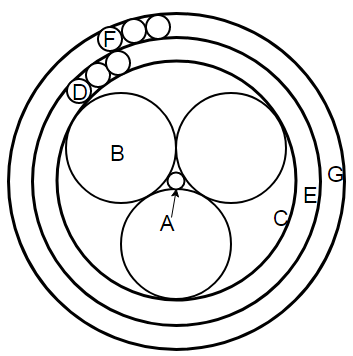
\includegraphics[scale=0.5]{figures/cross2}
\caption [$\; \:$ Cable cross-section in local model]{Illustration of cable cross-section in local model}
 \label{fig:crosspro}
\end{figure}
\noindent The cable consists of the upper 5 pitch lengths of the cable, and consists of several layers as displayed in the Figure above. The model was built up form the inner layer and outwards. 
The straight components are modeled with HSHEAR363 elements. That includes the inner core (A), the sheath around the conductors (C), the tape between the armouring layers (E), and the outer sheath(G). The helical components are modeled with HSHEAR353 elements and include the conductors (B) and the armouring layers (D) and (F). The cable is built out of one central node system, and all the components are connected to this node system in addition to having their own radial node system.\\\\ To model the contact between element groups, contact elements are used.  HCONT463 was used to describe the contact between different layers. The purpose of the element is connecting two other elements, making one of them the master and the other the slave. The modeling started in the inner layer of the cross-section, the core, and this was the first master element. The element connected the radial node of the core to the radial nodes of the conductors. Then the conductors were the master element and sheath 1 was the slave element. This continued until the outer sheath was reached. A description of how the different layers were connected to each other by the HCONT463 is illustrated in Figure \ref{fig:contact}

\begin{figure}[H]
\centering
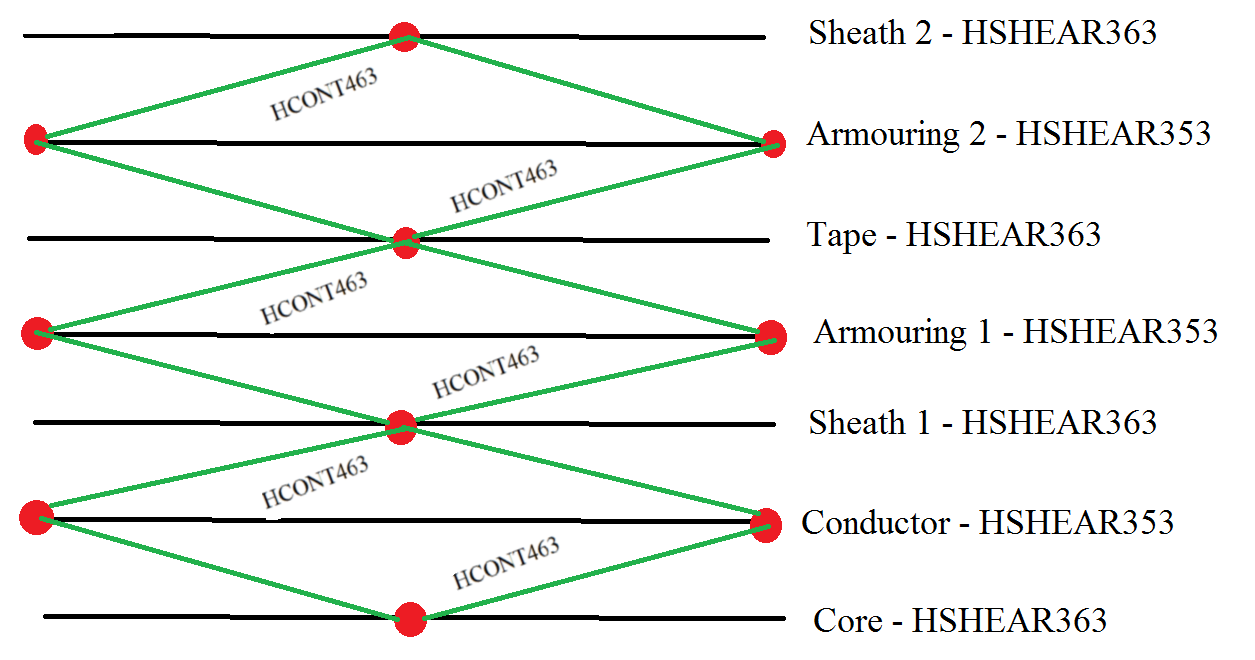
\includegraphics[scale=0.5]{figures/contact}
\caption[$\; \:$ Logic of HCONT463]{The element types for the different components in the cross section and the logic of HCONT463}
 \label{fig:contact}
\end{figure}

\noindent To describe the contact between the conductors, the element HCONT454 was used. This element connects the two radial nodes of the HSHEAR353 elements together.\newline
\newline
The conductors were modeled with a lay angle of 8 degrees, and the armouring has a lay angle of 20 degrees. The local model is 5 pitch lengths for the conductor. 1 pitch length can be calculated as:

 \begin{equation}
   L_p = \frac{2\pi R}{\tan(\alpha)}
\end{equation}
 Where $L_p$ is 1 pitch length, R is the radius in polar coordinates, and $\alpha$ is the lay angle\newline
 \newline
 With a lay angle of 8 degrees, 5 pitch lengths are calculated to be $L_p=3.35$m \newline
\newline
The cable includes three different materials, where the conductors are of copper, the armouring are of steel and the sheaths and tape are made of plastic. The most important material properties are reproduced in table \ref{table:matprop}
\begin{table} [H]
\centering
\begin{tabular}{ |c|c|c|c|}
\hline
Property &Steel & Copper  & Plastic \\
 \hline
 \hline
Type & Linear & Linear & Elastic\\
Young's modulus [GPA] & 210 & 115 & 0.7\\
Shear modulus [GPA]& 80 & 40 &  \\
Poisson's number [-]& 0.30 & 0.36 & 0.35\\
Axial stiffness [N]& 1.48e+06 & 1.07e+07 & \\
Bending stiffness [Nm$^2$] & 0.835 & 4.19 &\\
Torsional stiffness & 0.64 & 0.32&\\
 \hline
\end{tabular}
\caption{Properties of the materials used in the local model}
\label{table:matprop}
\end{table}


\noindent The friction between layers were determined by the use of FRICONTACT materials. Three different friction models (FRICONTACT materials) were used to model the friction between the layers. 

\begin{table} [H]
\centering
\begin{tabular}{ |c|c|c|c|}
\hline
Property &contact01 & contact1  & contact10 \\
 \hline
 \hline
Type & Coulomb friction & Coulomb friction & Coulomb friction\\
Static friction coeff. [-] & 0.15 & 0.15 & 0.15\\
Dynamic friction coeff. [-] & 0.15 & 0.15 & 0.15\\
Elastic stiffness in axial direction [N/m^$^2$] & 100e6 & 100e6 & 100e6 \\
Elastic stiffness in transv. direction [N/m^$^2$]& 100e6 & 100e6 & 100e6 \\
Surface stiffness [N/m$^2$] & 100e5 & 100e6 & 100e8\\
 \hline
\end{tabular}
\caption{Properties of the friction elements used in the local model}
\label{table:friprop}
\end{table}

The different friction models for the different contacts are described in table \ref{table:frimod}

\begin{table} [H]
\centering
\begin{tabular}{ |c|c|}
\hline
Contact & Friction Model  \\
 \hline
 \hline
Core - Conductor & contact01\\
Conductor - Conductor & contact1\\
Conductor - Sheath & contact1\\
Sheath 1 - Armouring 1 & contact1\\
Armouring 1 - Tape &contact10\\
Tape - Armouring 2 &contact10\\
Armouring 2 - Sheath 2 & contact1\\
 \hline
\end{tabular}
\caption{Friction models for different contacts in cable}
\label{table:frimod}
\end{table}

\subsection{Bend Stiffener}
To add more local stiffness to the flexible cable, a bend stiffener was added to the model. The following section is based on guidance from Professor Svein Sævik. 
\newline 
\newline
The dimensions of the bend stiffener are, for now, based on rough calculations and assumptions by the following equations: \newline
\newline

\noindent Locking radius of the flexible cable:
\begin{equation}
    LR = \frac{r}{1-F_j} = \frac{r}{1-0.9} = 10r
\end{equation}
Where LR is the locking radius, r is the radius of the conductor, $F_j$ is the fillfactor = 0.9 according to professor Svein Sævik. \newline
\newline
Minimum bend radius from \cite{API2014}:
\begin{equation}
   r_{min}= 1.5 * 1.1 * LR
\end{equation}
Where $r_{min}$ is the minimum locking radius, and LR is the locking radius. 
\newline
\newline
Max curvature:
\begin{equation}
   \kappa_{max}= \frac{1}{r_{min}}
\end{equation}
Where $\kappa_{max}$ is the maximum curvature, and  $r_{min}$ is the minimum locking radius.
\newline
\newline
Angle between cable and vessel: 
\begin{equation}
   \theta_{tot} = \theta_{s} + \theta_{p} +   \theta_{offset}
\end{equation}
Where $\theta_{tot}$ is the total angle at the end of the flexible cable, $\theta_{s}$ is angle due to surge, $\theta_{p}$ is angle due to pitch and $\theta_{offset}$ is the angle due to the offset of the floater. These variables are calculated as follows:\newline
\newline 
Angle due to surge:
\begin{equation}
   \theta_{s} = \arctan{(\frac{\mu_{surge}}{L_{1}})}
\end{equation}

\begin{equation}
   \mu_{surge} = \frac{H_{max}}{2} RAO
\end{equation}
Where L{1} is the assumed length from the vessel to the curve on the lazy wave configuration due to the buoyancy elements.  $H_{max}$ is the significant wave height for the most extreme sea state in the scatter diagram in Figure \ref{fig:scatn} and RAO is the response amplitude operator for surge provided by Dr. Techn. Olav Olsen. \newline
\newline 
\noindent Angle due to pitch:
\begin{equation}
   \theta_{pitch} = \frac{H_{max}}{2} RAO
\end{equation}
Where $H_{max}$ is the significant wave height for the most extreme sea state in the scatter diagram in figure \ref{fig:scatn} and RAO is the response amplitude operator for pitch provided by Dr. Techn. Olav Olsen. \newline
\newline
Angle due offset:
\begin{equation}
   \theta_{offset} = \arctan{(\frac{offset * depth}{L_1})}
\end{equation}
This can be used to calculate the length of the bend stiffener:

\begin{equation}
   L_{BS} = \frac{\theta_{max}}{\kappa_{max}} 
  \end{equation}
Where $L_{BS}$ is the length of the bend stiffener, $\theta_{max}$ is the maximum angle and $\kappa_{max}$ is the maximum curvature. \newline
\newline
Further, the outer diameter for the widest part of the bend stiffener can be calculated as follows: \newline
\newline 
Max tension is estimated to 
\begin{equation}
   T = 1.3  T_{static}
\end{equation}
Where T is the max tension, and $T_{static}$ is the static tension due to the configuration of the riser.

\begin{equation}
   T_{static} = 10 + W_s + L_1
\end{equation}
Where $W_s$ is the submerged weight of the cable and $L_1$ is the depth from the floater to the curve on the lazy wave configuration due to the buoyancy elements.\newline
\newline
\noindent $W_s$ was calculated for all the components pr meter cable the following way:

\begin{equation}
   W_s = \sum V (\rho_{comp}-\rho_{water})
\end{equation}
 Where V is the volume for each component, $\rho_{comp}$ is the density of the material of the component and $\rho_{water}$ is the density of the water.\\\\ Number of armouring fibres that fit around the cross section, the following method was used: 

 \begin{equation}
   F_j=\frac{n D}{\cos{(\alpha)} 2 \pi R}
\end{equation}
Where $F_j$ is the fill factor, n is the number of armouring fibers with diameter D  that can fit around a larger circle with radius R, and $\alpha$ is the lay angle of the armouring fibers.  \newline
\newline 
The bending stiffness EI was calculated by the following expression:

 \begin{equation}
   \kappa_{max} = \sqrt{\frac{T_{max}}{EI}}\theta_{max}
\end{equation}
Where $\kappa_{max}$ is the maximum curvature, $T_{max}$ is the maximum tension, EI is the bending stiffness, and $\theta_{max}$ is the maximum angle.\newline  
\newline 
\noindent Finally, the outer radius of the bend stiffener was calculated by:

 \begin{equation}
  EI = \frac{\pi}{4}(r_o^4 - r_i^4) 
\end{equation}
 Where EI is the bending stiffness, $r_o$ is the outer radius of the bend stiffener and $r_i$ is the inner radius.\newline 
\newline 
This gives the final dimensions for the bend stiffener: 
 \begin{table} [H]
\centering
\begin{tabular}{ |c|c|}
\hline
Parameter & Value [m] \\
 \hline
 \hline
 
 Length & 0.325 \\
 
Outer diameter, widest part & 0.3152\\

Outer diameter, narrowest part & 0.1\\

 Inner diameter & 0.0966 \\
 

 \hline
\end{tabular}
\caption{Dimensions of bend stiffener}
\label{table:dim}
\end{table}
\noindent The bend stiffener begins 1 pitch length away from the upper end of the cable, and is made out of polyurethane. It is modeled by the use of CROSSECTION command in BFLEX making the inclination very easy to model.  

\subsubsection{Material data for Bend Stiffener}
The material of the bend stiffener is a polymer with non-linear material properties.The initial Young's modulus was chosen to be 150 GPa, with a decay in stiffness according to  Figure \ref{fig:matbend}. The material was chosen in agreement with guidance from Professor Svein Sævik. 

\begin{figure}[H]
\centering
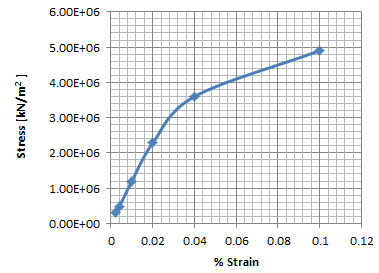
\includegraphics[scale=1]{figures/matbend}
\caption[$\; \:$ Stress-strain relationship for bend stiffener material]{Stress-strain relationship for bend stiffener material}
 \label{fig:matbend}
\end{figure}

\subsection{Stiff Pipe}
A stiff pipe was modeled at the very end of the cable. This was done to make sure that there was no curvature in the termination of the cable to avoid transient effects. The pipe has the length of one pitch length and was modeled with PIPE31 elements. The nodes of the stiff pipe are connected with the central node system of the cable through the CONSTR card in BFLEX. The card assigns one node to be the slave and the other to be master, and defines the relationship between them:
\begin{equation}
r_{Si}=C_1 \cdot r_{Mj}    
\end{equation}
Where $r_{Si}$ is the displacement of the slave node,  $C_1$ is a constant describing the relationship between the master and the slave and $r_{Mj}$ is the displacement of a master node.\newline 
\newline 
In this case $C_1$ is 1, so the nodes will follow each other exactly. 

\subsection{Boundary Conditions}
The boundary conditions for the cable is created in such a way that the cable can slide inside the bend stiffener. The following constraints are made for the different components:
\begin{itemize}
    \item Centroid system: Fixed in 2 and 6 for all nodes, and 2 and 3 for the last nodes
    \item Radial nodes of the core, sheaths, and tape are fixed in 2 and 3 for all nodes. 
    \item The conductors are fixed in 1 and 2 for the first and last node. Degree of freedom 4 is fixed in all nodes.
    \item The armouring layers are fixed in 1 at the first node, and in 2,4,5 and 6 for all nodes
\end{itemize}

\section {Testing}
\label{sec:localtest}
To make sure the global and local model were acceptable, some key features had to be checked before the analyses could begin. 
\subsection{Testing of Global Model}
To make sure the global model was ready to be used in further analyses, several things were investigated. The design criteria for the global model was that the curvature could not exceed $\kappa=1.3675$ anywhere in the cable to avoid locking of the cable. To test this, the most severe sea state according to the scatter diagram for West of Barra in Figure \ref{fig:scatn} was tested in a dynamic analysis. The key variables used in the test are displayed in table \ref{table:testglob}.

\begin{table} [H]
\centering
\begin{tabular}{ |c|c|c|}
\hline
Variable & Value \\
 \hline
 \hline
Hs [m] & 13.5\\
Tp[s] & 16 \\
Time step [s] & 0.1 \\
 \hline
\end{tabular}
\caption{Key variables used in testing of global model}
\label{table:testglob}
\end{table}

The following results for the three wind conditions were seen as interesting to assess the quality of the model:
\begin{itemize}
    \item The static configuration, to make sure the cable had the desired steep S shape, and that the buoyancy section is not too high in the water.
    \item Curvature envelope, to make sure the curvature does not exceed the max curvature of 1.3675 $\frac{1}{m}$
    \item Max force envelope, to make sure the tension in the cable is acceptable
    \item Min force envelope, to make sure the there is no compression in the bottom of the cable
\end{itemize}

\subsection{Results from Testing of Global Model}
The static configuration without current for the three different wind conditions: 
\begin{figure}[H]
\subfloat[Near position\label{fig:cavS200}]
  {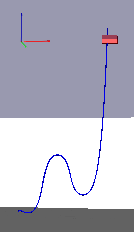
\includegraphics[width=.3\linewidth]{figures/statposnear}}\hfill
\subfloat[Neutral position \label{fig:cavS2500}]
  {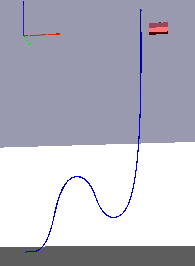
\includegraphics[width=.3\linewidth]{figures/statposneu}}\hfill
  \subfloat[Far position \label{fig:cavS5000}]
  {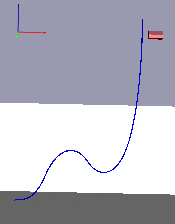
\includegraphics[width=.3\linewidth]{figures/statposfar}}\hfill
\caption{Static configuration for the global model for different wind conditions}
\label{fig:statcon}
\end{figure}

The static configuration with current for the three different wind conditions: 
\begin{figure}[H]
\subfloat[Near position\label{fig:cavS200}]
  {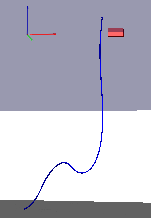
\includegraphics[width=.3\linewidth]{figures/statposnearc}}\hfill
\subfloat[Neutral position \label{fig:cavS2500}]
  {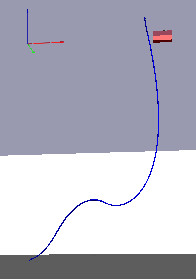
\includegraphics[width=.3\linewidth]{figures/statposneuc}}\hfill
  \subfloat[Far position \label{fig:cavS5000}]
  {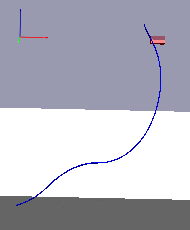
\includegraphics[width=.3\linewidth]{figures/statposfarc}}\hfill
\caption{Static configuration for the global model for different wind conditions}
\label{fig:statcon}
\end{figure}

\noindent These positions gave the following configurations for the dynamic cable without current: 
\begin{figure}[H]
\centering
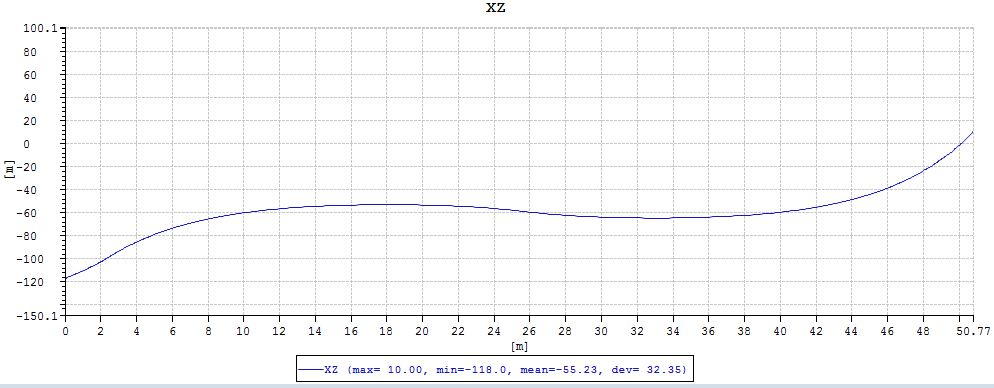
\includegraphics[scale=0.5]{figures/confignear}
\caption{Configuration for near position}
 \label{fig:confignear}
\end{figure}

\begin{figure}[H]
\centering
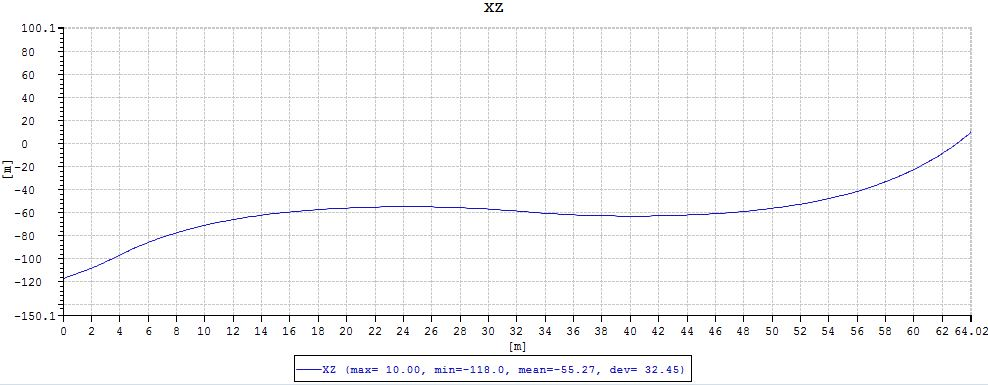
\includegraphics[scale=0.5]{figures/configneu}
\caption{Configuration for neutral position}
 \label{fig:configneu}
\end{figure}

\begin{figure}[H]
\centering
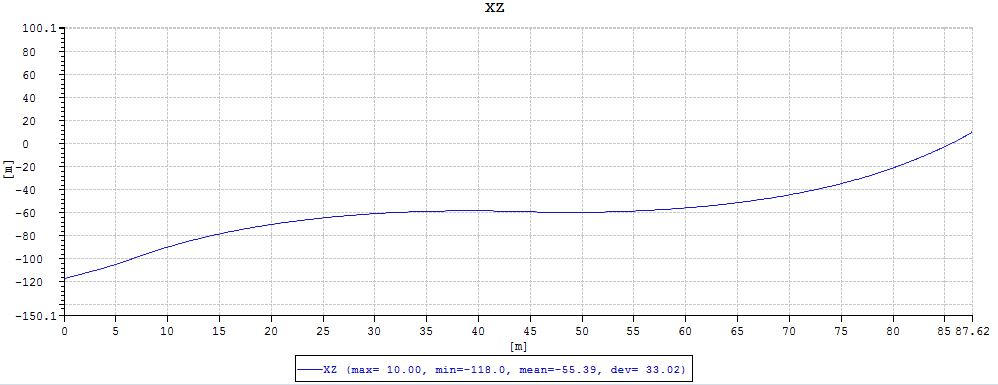
\includegraphics[scale=0.5]{figures/configfar}
\caption{Configuration for far position}
 \label{fig:configfar}
\end{figure}

\noindent These positions gave the following configurations for the dynamic cable with current: 
\begin{figure}[H]
\centering
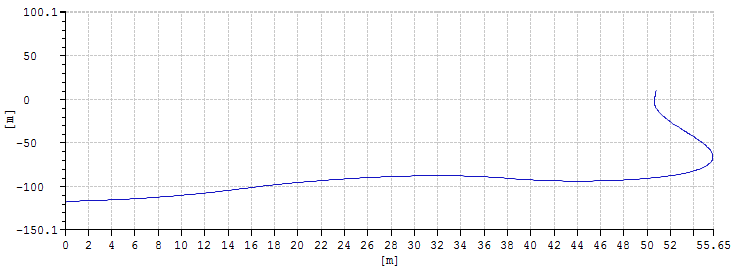
\includegraphics[scale=0.5]{figures/confignearc}
\caption{Configuration for near position}
 \label{fig:confignear}
\end{figure}

\begin{figure}[H]
\centering
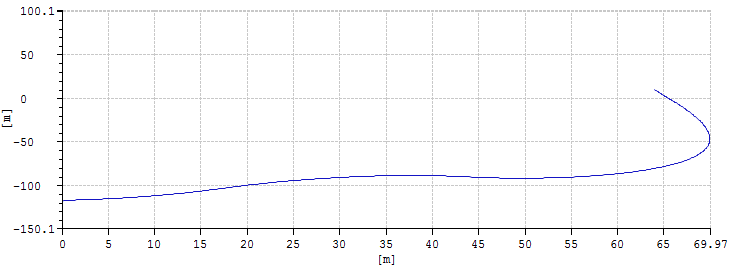
\includegraphics[scale=0.5]{figures/configneuc}
\caption{Configuration for neutral position}
 \label{fig:configneu}
\end{figure}

\begin{figure}[H]
\centering
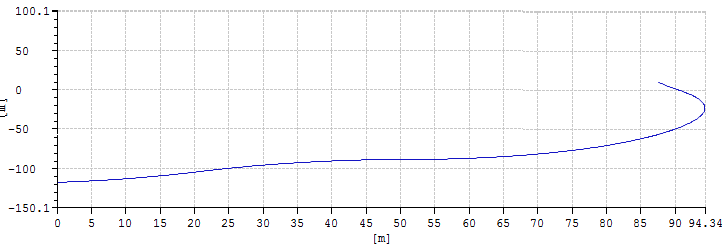
\includegraphics[scale=0.5]{figures/configfarc}
\caption{Configuration for far position}
 \label{fig:configfar}
\end{figure}

\noindent The envelope curves for the curvatures

\begin{figure}[H]
\centering
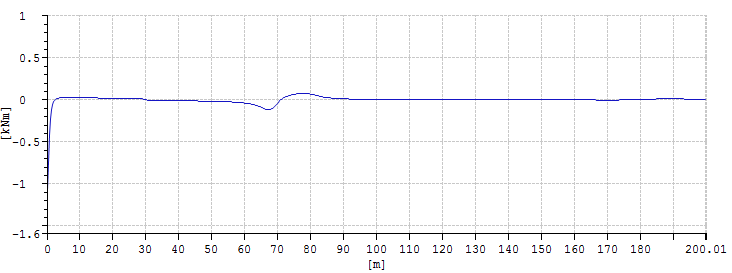
\includegraphics[scale=0.5]{figures/envcurvenear}
\caption{Curvature envelope for near position}
 \label{fig:envcurvenear}
\end{figure}

\begin{figure}[H]
\centering
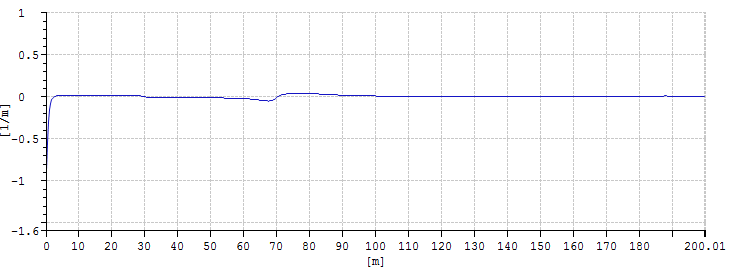
\includegraphics[scale=0.5]{figures/envcurveneu}
\caption{Curvature envelope for neutral position}
 \label{fig:envcurveneu}
\end{figure}

\begin{figure}[H]
\centering
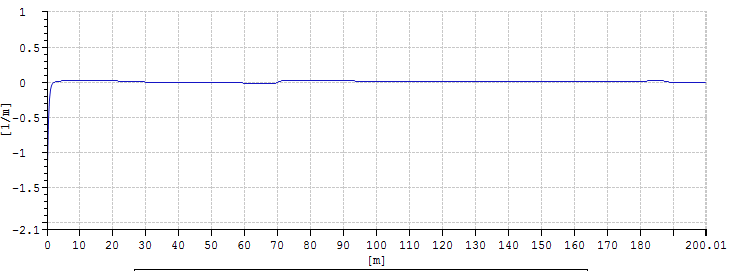
\includegraphics[scale=0.5]{figures/envcurvefar}
\caption{Curvature envelope for far position}
 \label{fig:envcurvefar}
\end{figure}

\noindent The max tension over the length of the cable

\begin{figure}[H]
\centering
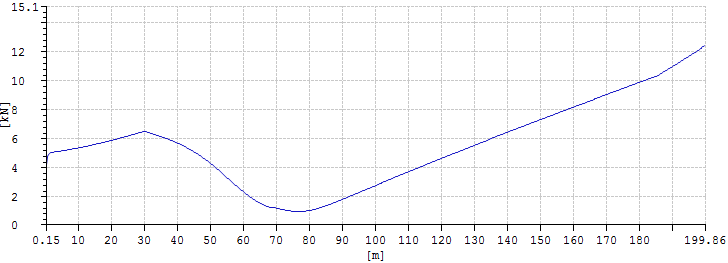
\includegraphics[scale=0.5]{figures/fmaxnear}
\caption{The max tension over the length of the cable in near position}
 \label{fig:fmaxnear}
\end{figure}


\begin{figure}[H]
\centering
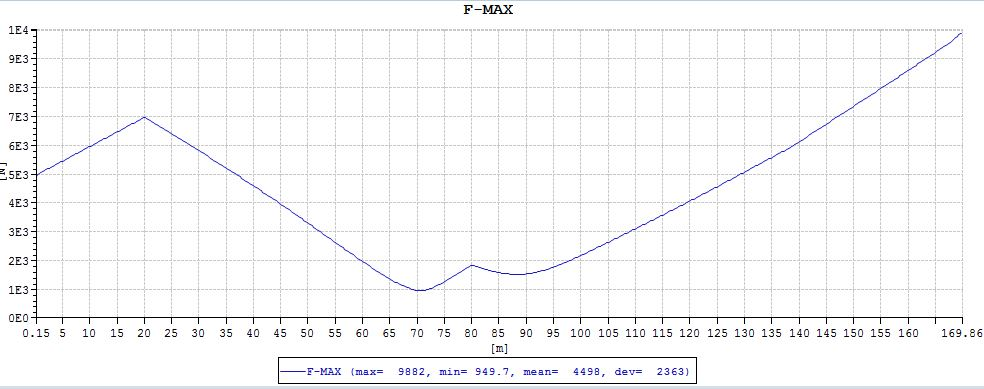
\includegraphics[scale=0.5]{figures/fmaxneu}
\caption{The max tension over the length of the cable in neutral position}
 \label{fig:fmaxneu}
\end{figure}


\begin{figure}[H]
\centering
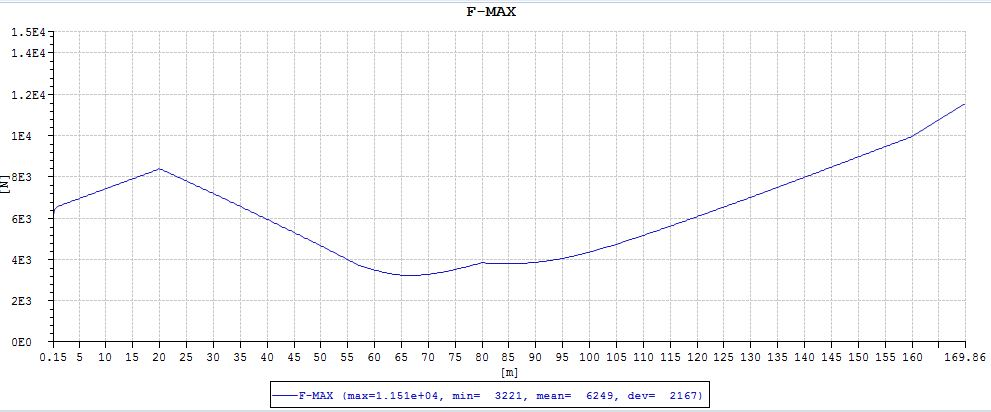
\includegraphics[scale=0.5]{figures/fmaxfar}
\caption{The max tension over the length of the cable in far position}
 \label{fig:fmaxfar}
\end{figure}

\noindent The minimum tension over the length of the cable

\begin{figure}[H]
\centering
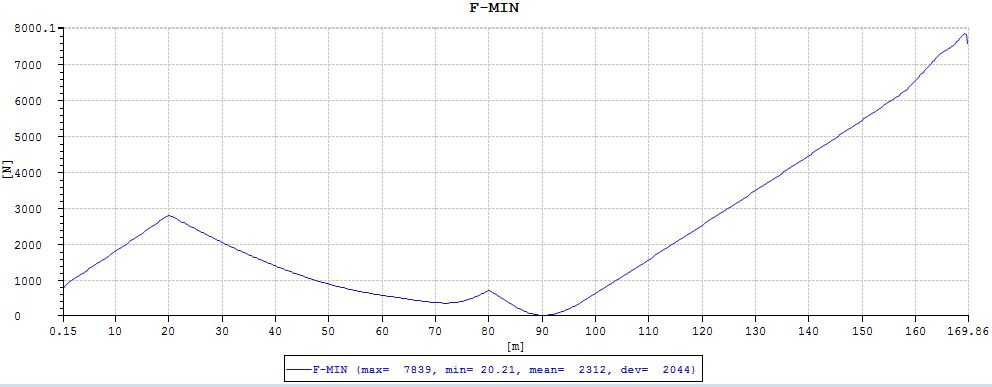
\includegraphics[scale=0.5]{figures/fminnear}
\caption{The minimum tension over the length of the cable in near position}
 \label{fig:fminnear}
\end{figure}


\begin{figure}[H]
\centering
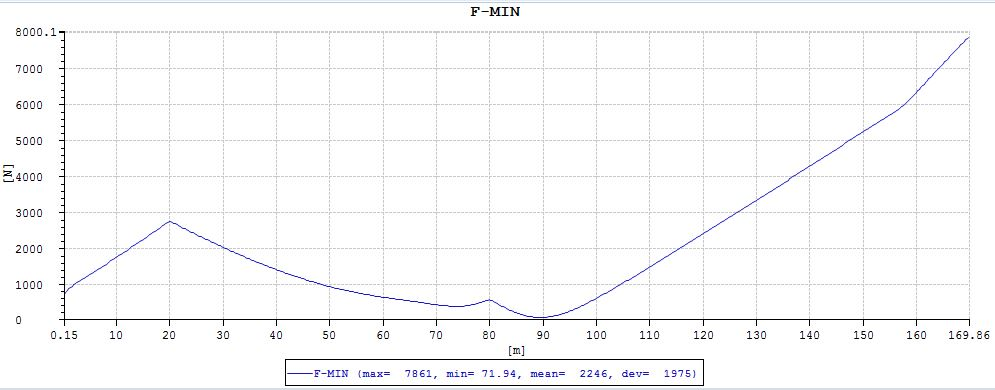
\includegraphics[scale=0.5]{figures/fminneu}
\caption{The minimum tension over the length of the cable in neutral position}
 \label{fig:fminneu}
\end{figure}


\begin{figure}[H]
\centering
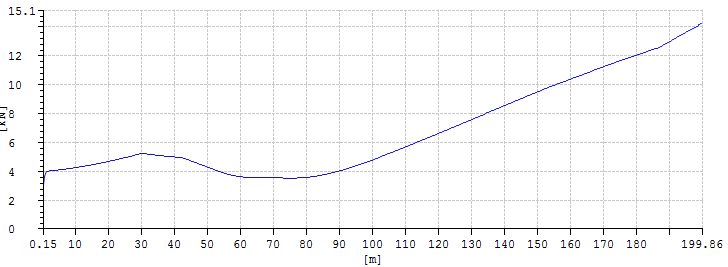
\includegraphics[scale=0.5]{figures/fminfar}
\caption{The minimum tension over the length of the cable in far position}
 \label{fig:fminfar}
\end{figure}



\subsection{Testing of Local Model}
The local model was, as the global model tested to see if it performs in a satisfactory manner. The following figures show the local model and some of its components:

\begin{figure}[H]
\subfloat[Local model from the side with bend stiffener \label{fig:lm_total}]
  {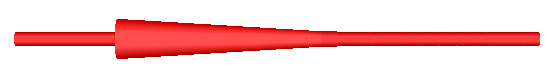
\includegraphics[width=.45\linewidth]{figures/lm_total}}\hfill
\subfloat[Cable cross section in local model \label{fig:lm_cross}]
  {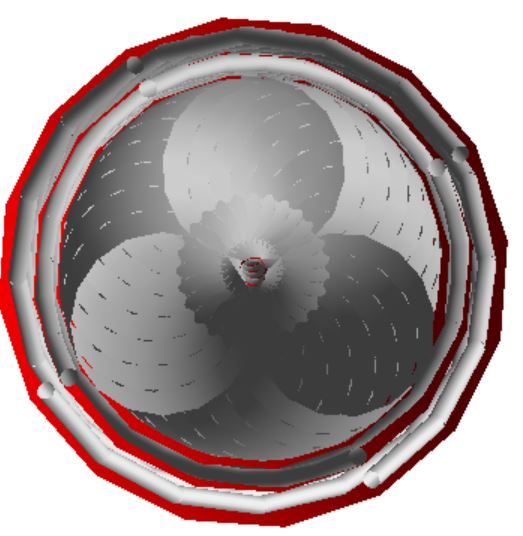
\includegraphics[width=.25\linewidth]{figures/lm_cross}}\hfill
\caption{Local model}
\label{fig:volt}
\end{figure}

\begin{figure}[H]
\subfloat[Conductors \label{fig:single}]
  {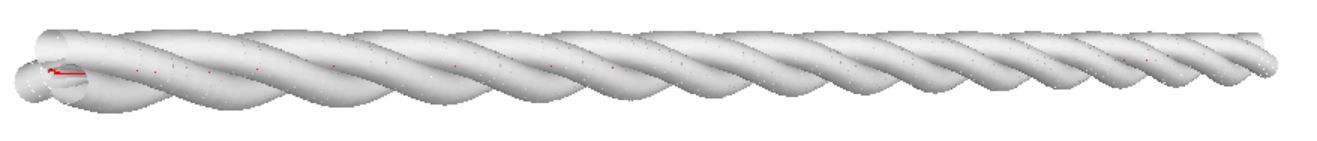
\includegraphics[width=.45\linewidth]{figures/lm_conductors}}\hfill
\subfloat[Armouring \label{fig:3phase}]
  {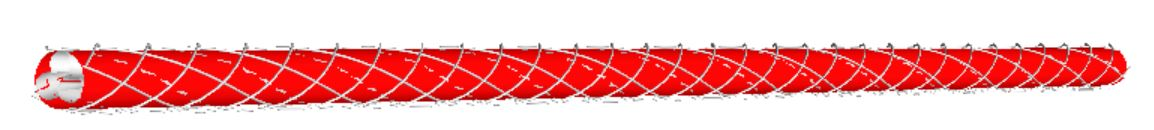
\includegraphics[width=.45\linewidth]{figures/lm_arm}}\hfill
\caption{Helical components in the local model}
\label{fig:volt}
\end{figure}
 \noindent The following sequence of loads was added to the local model.
\begin{enumerate}
    \item Gravity Load: Gravity is turned off on the local model, but the effect of the mass of the model should still be applied. This was added at the very first time step.
    \item Tension: Tension was added to the local model in the axial direction on the last node in the outer sheath, with magnitude 50kN. The load was applied at t=1s to t=5s. seconds
    \item Initial strain: Initial strain was added to the outer sheath of the model in 1 direction. The strain was added to all the elements with a magnitude 0.03. It was applied at t=1s to t=5s.
    \item Bending: Smooth bending of the cable was applied. The cable was bent from 0 degrees to 5 degrees between t=5 and t=15, and from 5 degrees to -5 degrees between t=15 and t=35.  
\end{enumerate}
 



